% ============================================================================
\section{Thực nghiệm và đánh giá}
\label{sec:experiments}
% ============================================================================

\begin{keybox}
\textbf{Nguồn của chương này.} Mọi con số trong chương được sinh tự động từ các tệp
\code{results/*.json} (Phụ lục~\ref{app:trace}); không con số kết quả nào được gõ tay. Chương đi
theo thứ tự: dữ liệu và công cụ đo (\ref{sec:data}--\ref{sec:alignment-res}), kết quả tổng
(\ref{sec:res-main}), rồi lần lượt bốn câu hỏi nghiên cứu (\ref{sec:res-rq1}--\ref{sec:res-rq4}).
\end{keybox}

\subsection{Môi trường}
\label{sec:env}

\begin{table}[htbp]
\centering
\caption{Môi trường phần cứng và phần mềm}
\label{tab:env}
\renewcommand{\arraystretch}{1.13}
\small
\begin{tabular}{@{}l l@{}}
\toprule
\textbf{Thành phần} & \textbf{Cấu hình} \\
\midrule
Máy tính & Apple M5 Pro, 18 nhân, 48 GB bộ nhớ hợp nhất, macOS 26.4.1 \\
Thiết bị tính toán & GPU tích hợp qua PyTorch MPS \\
Ngôn ngữ, môi trường & Python 3.12, \code{uv} \\
Học sâu & PyTorch 2.14.0 \cite{paszke2019pytorch}; \code{transformers} 5.17.0 \cite{wolf2020transformers}; \code{tokenizers} 0.23.2 \\
Tách từ & \code{pyvi} 0.1.1 \\
Học máy cổ điển & scikit-learn 1.9.1 \cite{pedregosa2011sklearn} \\
Kiểm thử, hình & pytest 9.1.1; Matplotlib 3.11.2 \\
\bottomrule
\end{tabular}
\end{table}

\subsection{Dữ liệu}
\label{sec:data}

UIT-ViQuAD~2.0 được tải từ HuggingFace (\code{taidng/UIT-ViQuAD2.0}) bằng
\code{scripts/fetch\_data.py}. Các số trong Bảng~\ref{tab:data} được đo trực tiếp từ tệp đã
tải; độ dài tính theo âm tiết (tách theo khoảng trắng).

\begin{table}[htbp]
\centering
\caption{Dữ liệu dùng trong đồ án}
\label{tab:data}
\renewcommand{\arraystretch}{1.15}
\footnotesize
\begin{tabularx}{\textwidth}{@{}L r r r r@{}}
\toprule
& \textbf{train (gốc)} & \textbf{fit} & \textbf{dev} & \textbf{validation = test} \\
\midrule
Vai trò & --- & huấn luyện & chọn epoch & chấm một lần \\
Số câu hỏi & \NTrain & \NFit & \NDev & \NVal \\
Số đoạn văn & \NTrainCtx & \NFitCtx & \NDevCtx & \NValCtx \\
Câu không có đáp án & \NTrainImp{} (\PctTrainImp\%) & \NFitImp{} (\PctFitImp\%) & \NDevImp{} (\PctDevImp\%) & \NValImp{} (\PctValImp\%) \\
Câu có đáp án & \NTrainAns & \NFitAns & \NDevAns & \NValAns \\
\midrule
Đoạn văn (âm tiết): TB / trung vị / max & 179,0 / 160 / 1.537 & & & 167,6 / 152 / 618 \\
Đáp án (âm tiết): TB / trung vị / p95 & 9,95 / 6 / 31 & & & 9,81 / 6 / 30 \\
\bottomrule
\end{tabularx}
\end{table}

Tỉ lệ câu không có đáp án của validation là \PctValImp\%: đó chính là điểm EM của một hệ thống
\emph{không làm gì cả} và luôn trả về chuỗi rỗng. Mọi con số dưới đây phải được đọc so với mức
sàn này.

\paragraph{Hai tokenizer nhìn cùng dữ liệu khác nhau.} Trên 400 đoạn văn train lấy ngẫu nhiên,
PhoBERT (sau tách từ) sinh trung bình 171 token mỗi đoạn văn (p95: 306), XLM-R sinh 218 token
(p95: 389) --- chuỗi của PhoBERT ngắn hơn khoảng 22\% vì một token thường là cả một từ nhiều âm
tiết. Tuy vậy PhoBERT chỉ có 256 vị trí, nên 14\% đoạn văn cần hơn một cửa sổ, so với 7\% với
XLM-R ở độ dài 384. Lợi thế ``chuỗi ngắn hơn'' của mô hình word-level bị giới hạn vị trí triệt
tiêu một phần.

\subsection{Kiểm định bộ stress-test}
\label{sec:audit}

Bộ stress-test 250 câu được xây trong giai đoạn đầu của đồ án để cô lập năm cơ chế thất bại
(E1 ranh giới từ ghép, E2 ngữ cảnh gây nhiễu, E3 câu hỏi phủ định, E4 suy luận nhiều bước, E5
nhãn mập mờ). Theo giao thức ở Mục~\ref{sec:audit-method}, nó được kiểm định \emph{trước} khi
chấm mô hình. Kết quả (Bảng~\ref{tab:audit}, Hình~\ref{fig:audit}) cho thấy bộ này \textbf{không
dùng được để so sánh mô hình}.

\begin{table}[htbp]
\centering
\caption{Kiểm định tự động bộ stress-test (nguồn: \code{results/stress\_test\_audit.json})}
\label{tab:audit}
\renewcommand{\arraystretch}{1.15}
\footnotesize
\setlength{\tabcolsep}{3pt}
\resizebox{\textwidth}{!}{%
\begin{tabular}{@{}l >{\raggedright\arraybackslash}p{2.9cm} r r r r r r r@{}}
\toprule
& & & \textbf{Có} & \multicolumn{3}{c}{\textbf{Trong số câu có đáp án}} & \textbf{Câu hỏi} & \\
\cmidrule(lr){5-7}
& \textbf{Nhóm} & \textbf{Câu} & \textbf{đáp án} & \textbf{đ.án $\in$ ngữ cảnh} & \textbf{offset đúng} & \textbf{đ.án $\in$ câu hỏi} & \textbf{khác nhau} & \textbf{Hợp lệ} \\
\midrule
\tabinput{generated/tab_audit.tex}
\bottomrule
\end{tabular}}
\end{table}

\begin{figure}[htbp]
\centering
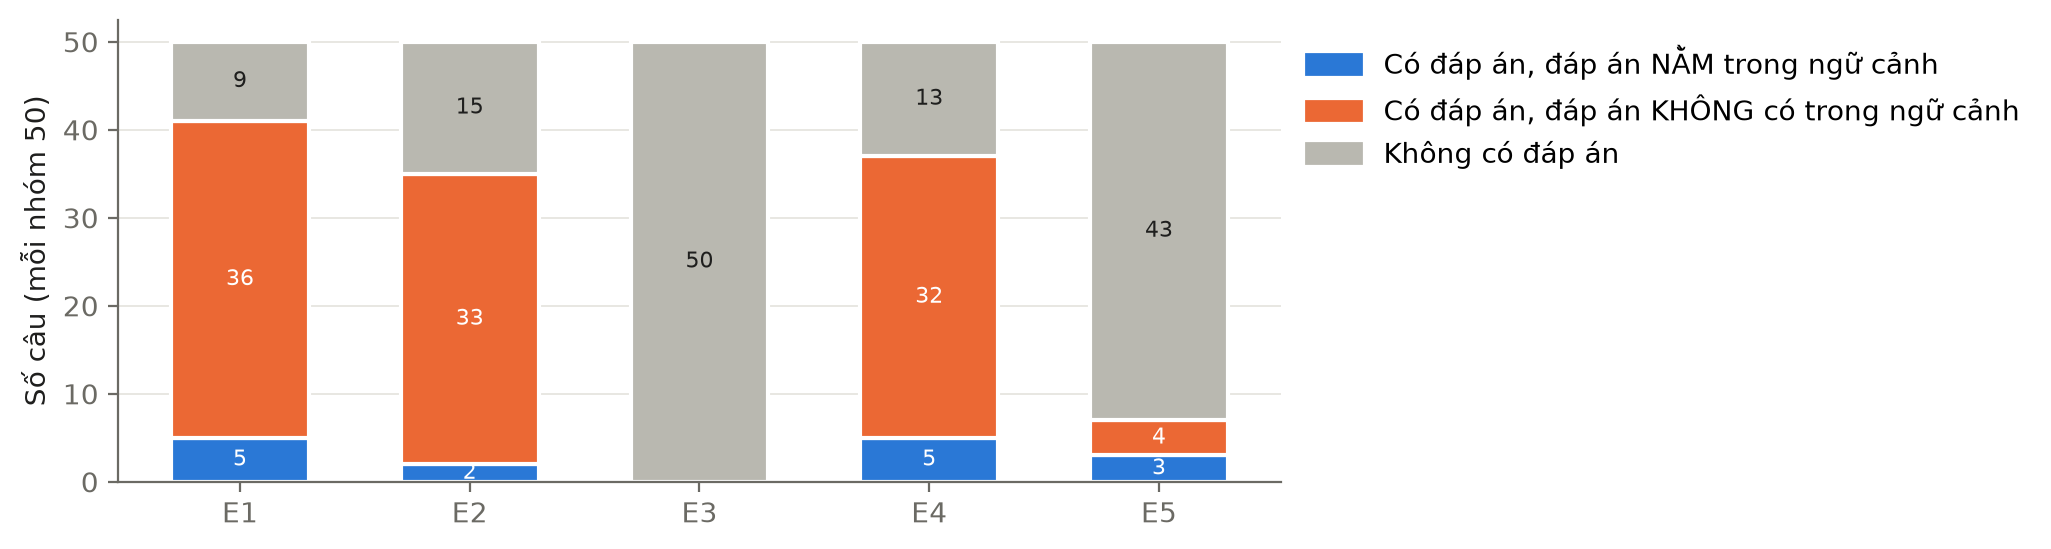
\includegraphics[width=0.88\textwidth]{figures/stress_audit.png}
\caption{Thành phần từng nhóm stress-test. Phần cam là câu có đáp án mà đáp án không nằm trong ngữ cảnh --- không mô hình trích xuất nào trả lời đúng được}
\label{fig:audit}
\end{figure}

Bốn phát hiện:

\begin{enumerate}
  \item \textbf{Đáp án không nằm trong ngữ cảnh.} Chỉ \AuditAnsInCtx{} trên \AuditAns{} câu có đáp
        án chứa đáp án vàng trong đoạn văn; chỉ \AuditOffsetOK{} câu có \code{answer\_start} đúng.
        Với các câu còn lại, điểm EM tối đa của \emph{mọi} mô hình trích xuất là 0.
  \item \textbf{Độ đa dạng rất thấp.} Cả 250 câu dùng chung \AuditCtx{} đoạn văn. Nhóm E5 có 50 câu
        nhưng chỉ \AuditEFiveDistinctQ{} câu hỏi khác nhau; nhóm E1 có \AuditEOneDistinctQ{}. Câu hỏi
        của E1 phần lớn là câu ``siêu ngôn ngữ'' dạng \emph{``Tại sao từ ghép `X' khó được tách từ
        chính xác trong ngữ cảnh này?''} với đáp án là chính X, nên 19 câu có đáp án nằm nguyên văn
        trong câu hỏi. Chúng đo khả năng chép lại cụm trong nháy đơn, không đo ranh giới từ ghép.
  \item \textbf{Mất cân bằng nhãn tạo điểm thoái hoá.} E3 có 100\% câu không có đáp án, E5 có 86\%.
        Hệ thống luôn từ chối đạt 100 điểm trên E3 và \AbstainStressEM{} điểm trên toàn bộ 250 câu.
  \item \textbf{Tệp gộp chứa bản ghi ngoài lược đồ.} Tệp \code{stress\_test\_combined.json} có
        \AuditCombined{} bản ghi: 250 câu SQuAD cộng \AuditFlat{} bản ghi ``phẳng'' không theo lược đồ
        SQuAD (24 mỗi nhóm) mà tài liệu dự án không nhắc tới. Đây là lời giải cho sự chênh lệch
        ``370 so với 250'' từng ghi nhận.
\end{enumerate}

\paragraph{Nguyên nhân gốc.} Truy ngược mã sinh dữ liệu (\code{legacy/stress\_test\_generator.py})
cho thấy hai lỗi ``sai âm thầm'' cụ thể: hàm \code{\_find\_answer\_start} trả về \textbf{0} khi không
tìm thấy đáp án trong ngữ cảnh thay vì báo lỗi; và hàm \code{\_wrap\_into\_squad} gán ngữ cảnh
\emph{theo vòng} cho các mẫu chưa có ngữ cảnh --- sau khi câu hỏi và đáp án đã được viết cho một
ngữ cảnh khác. Hai lỗi cộng lại tạo ra dữ liệu đúng định dạng, qua được mọi kiểm tra rò rỉ (báo cáo
rò rỉ đi kèm ghi \code{is\_clean: true}), nhưng sai về nội dung.

\paragraph{Hệ quả cho thiết kế.} Bộ stress-test được giữ lại \emph{như một đối tượng nghiên cứu},
không như một thước đo: các mô hình vẫn được chấm trên nó (Mục~\ref{sec:res-rq3}) để cho thấy điểm
số trên một bộ chẩn đoán lỗi trông như thế nào, nhưng không kết luận nào về mô hình dựa trên nó.
Vai trò chẩn đoán được chuyển sang các phép đo trên \emph{validation} --- \NValAns{} câu có đáp án do
người gán --- bắt đầu từ phép đo biên từ dưới đây. Đây đúng là điều kiện mà Bowman và Dahl
\cite{bowman2021fix} nêu: một bộ chẩn đoán chỉ có giá trị khi nhãn của nó đúng.

\subsection{Trần EM do biên từ}
\label{sec:alignment-res}

Phép đo ở Mục~\ref{sec:alignment} chạy trên toàn bộ \SegN{} câu có đáp án của validation, không cần
mô hình:

\begin{itemize}
  \item \textbf{\SegAligned{} câu (\SegAlignedPct\%)} có ít nhất một đáp án vàng khớp biên từ của
        \code{pyvi}. Chỉ \textbf{\SegMis{} câu (\SegMisPct\%)} có đáp án cắt ngang một từ (\SegStartCut{}
        câu cắt ở đầu, \SegEndCut{} câu cắt ở cuối).
  \item \textbf{Trần EM của một mô hình word-level hoàn hảo là \SegOracle\%}: kênh ``đơn vị đầu ra''
        của giả thuyết RQ1 chỉ lấy đi được tối đa \SegCeilingLoss{} điểm EM trên câu có đáp án.
  \item Trên chính \SegMis{} câu lệch biên, span nguyên-từ gần nhất vẫn đạt EM trong \SegOracleMis\%
        trường hợp, vì phần thừa chỉ là dấu câu mà bước chuẩn hoá xoá đi.
\end{itemize}

Đọc từng câu trong \SegMis{} câu lệch biên cùng kết quả tách từ xung quanh đáp án cho một bức tranh
khác hẳn giả thuyết (Bảng~\ref{tab:misaligned}): phần lớn \emph{không} phải là ranh giới từ ghép
khó của tiếng Việt, mà là \textbf{lỗi của bộ tách từ} và \textbf{lỗi gán nhãn}.

\begin{table}[htbp]
\centering
\caption{Phân loại \SegMis{} câu lệch biên từ trên validation (nguồn: \code{results/misaligned\_labels.json})}
\label{tab:misaligned}
\renewcommand{\arraystretch}{1.18}
\small
\begin{tabularx}{\textwidth}{@{}L r L@{}}
\toprule
\textbf{Nguyên nhân} & \textbf{Số câu} & \textbf{Ví dụ: tách từ quanh đáp án (\textbf{vàng})} \\
\midrule
\code{pyvi} dính dấu chấm vào token viết hoa (luật chữ viết tắt) & \MisPeriod & \code{như \textbf{CNN}.} $\to$ \code{CNN.}; \code{vua Ferdinand \textbf{VII}.} \\
\code{pyvi} nối nhầm âm tiết qua ranh giới từ & \MisMerge & \code{phim hoạt\_hình \textbf{Mỹ}\_Chú chuột}; \code{tại \textbf{Nam\_Phi}\_với} \\
Lỗi gán nhãn: đáp án vàng bị cắt giữa âm tiết & \MisAnnot & vàng ``\textbf{o thời gian} \dots'' (thiếu ``d''); ``\dots các nhà \textbf{thông thá}'' \\
Ranh giới từ ghép thật & \MisCompound & \code{bởi\_\textbf{vì}}; \code{vào\_\textbf{khoảng}} \\
\bottomrule
\end{tabularx}
\end{table}

\begin{keybox}
\textbf{Hệ quả cho RQ1.} Kênh ``PhoBERT không thể trả lời nửa từ'' giải thích được \emph{tối đa}
\SegCeilingLoss{} điểm EM trên câu có đáp án, và chỉ \MisCompound{} trong \SegMis{} câu lệch biên là ranh
giới từ ghép thật. Nếu PhoBERT kém XLM-R nhiều hơn mức đó, phần chênh còn lại phải đến từ kênh khác ---
biểu diễn, dữ liệu tiền huấn luyện, giới hạn 256 vị trí --- chứ không phải từ việc đáp án cắt ngang từ
ghép. Ngược lại, các lỗi của \code{pyvi} ở bảng trên (nối nhầm âm tiết, dính dấu câu) là những lỗi
\emph{cũng xảy ra bên trong ngữ cảnh}, và chúng đi vào biểu diễn đầu vào của PhoBERT ở mọi câu, không
chỉ ở câu lệch biên.
\end{keybox}
